\documentclass[a4paper, 12pt]{article}
\addtolength{\topmargin}{-2in}
\addtolength{\textheight}{2in}
\addtolength{\oddsidemargin}{-.4in}
\addtolength{\textwidth}{.8in}

\usepackage[french]{babel}

%% \usepackage{lastpage}
%% \usepackage{fancyhdr}
%% \fancypagestyle{plain}{%
%%   \fancyfoot[C]{\thepage{}/\pageref{LastPage}}
%% }
%% \renewcommand{\headrulewidth}{0pt}
%% \pagestyle{plain}

\usepackage[bitstream-charter]{mathdesign}
\usepackage{fontspec}
%% \setmainfont{Charter}
\setmonofont[Scale=MatchLowercase]{Fira Mono}

\usepackage{graphicx}

\usepackage{listings}
\lstset{basicstyle=\ttfamily}
\lstset{tabsize=2, columns=fullflexible, keepspaces=true}
\lstset{breaklines=false, showstringspaces=false}
\lstset{frame=leftline, framerule=1pt}
\lstset{framesep=4pt}

\title{Quiz HTML \& CSS}
\author{U.V. Domaine}
\date{28 septembre 2018}

\begin{document}

\maketitle

\textbf{Nom} :

Sans machine ni document

Durée : 5 minutes

\vspace{1cm}

\begin{enumerate}
\item Expliquez comment HTML et CSS sont utilisés par les navigateurs pour
  présenter une page web à l'utilisateur.

  \framebox(400,80){}

\item Corrigez l'extrait HTML qui suit:
\begin{lstlisting}
<main id=first>
  <h2>Section 1</h3>
  <a href="http://en.wikipedia.org/" Wikipedia>
<main>
\end{lstlisting}

\framebox(400,80){}

\item Entourez tous les éléments HTML ciblés par le sélecteur CSS
  \lstinline{section > p a}

  \vspace{.2in}
  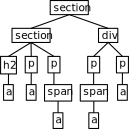
\includegraphics[width=6cm,keepaspectratio]{quiz1-tree}

\end{enumerate}

\end{document}
